
\documentclass[12pt, a4paper]{report}
\usepackage{epsfig}
\usepackage{subfigure}
%\usepackage{amscd}
\usepackage{amssymb}
\usepackage{graphicx}
%\usepackage{amscd}
\usepackage{amssymb}
\usepackage{subfiles}
\usepackage{framed}
\usepackage{subfiles}
\usepackage{amsthm, amsmath}
\usepackage{amsbsy}
\usepackage{framed}
\usepackage[usenames]{color}
\usepackage{listings}
\lstset{% general command to set parameter(s)
basicstyle=\small, % print whole listing small
keywordstyle=\color{red}\itshape,
% underlined bold black keywords
commentstyle=\color{blue}, % white comments
stringstyle=\ttfamily, % typewriter type for strings
showstringspaces=false,
numbers=left, numberstyle=\tiny, stepnumber=1, numbersep=5pt, %
frame=shadowbox,
rulesepcolor=\color{black},
,columns=fullflexible
} %
%\usepackage[dvips]{graphicx}
\usepackage{natbib}
\bibliographystyle{chicago}
\usepackage{vmargin}
% left top textwidth textheight headheight
% headsep footheight footskip
\setmargins{3.0cm}{2.5cm}{15.5 cm}{22cm}{0.5cm}{0cm}{1cm}{1cm}
\renewcommand{\baselinestretch}{1.5}
\pagenumbering{arabic}
\theoremstyle{plain}
\newtheorem{theorem}{Theorem}[section]
\newtheorem{corollary}[theorem]{Corollary}
\newtheorem{ill}[theorem]{Example}
\newtheorem{lemma}[theorem]{Lemma}
\newtheorem{proposition}[theorem]{Proposition}
\newtheorem{conjecture}[theorem]{Conjecture}
\newtheorem{axiom}{Axiom}
\theoremstyle{definition}
\newtheorem{definition}{Definition}[section]
\newtheorem{notation}{Notation}
\theoremstyle{remark}
\newtheorem{remark}{Remark}[section]
\newtheorem{example}{Example}[section]
\renewcommand{\thenotation}{}
\renewcommand{\thetable}{\thesection.\arabic{table}}
\renewcommand{\thefigure}{\thesection.\arabic{figure}}
\title{Research notes: linear mixed effects models}
\author{ } \date{ }


\begin{document}
\author{Kevin O'Brien}
\title{Mixed Models for Method Comparison Studies}
\tableofcontents






\chapter{Appendices}


\section{Outline of Thesis}
Thus the study of method comparison is introduced. The intention of this thesis is to progress the
study of method comparison studies, using a statistical method known as Linear mixed effects models.
Chapter two shall describe linear mixed effects models, and how the use of the linear mixed
effects models have so far extended to method comparison studies. Implementations of important existing work shall be presented, using the \texttt{R} programming language.

Model diagnostics are an integral component of a complete statistical analysis.
In chapter three model diagnostics shall be described in depth, with particular
emphasis on linear mixed effects models, further to chapter two.

For the fourth chapter, important linear mixed effects model diagnostic methods shall be extended to method comparison studies, and proposed methods shall be demonstrated on data sets that have become well known in literature on method comparison. The purpose is to both calibrate these methods and to demonstrate applications for them.
The last chapter shall focus on robust measures of important parameters such as agreement.
	\section{Alternative Agreement Indices}
	As an alternative to limits of agreement, \citet{lin2002} proposes the use of
	the mean square deviation in assessing agreement. The mean square
	deviation is defined as the expectation of the squared differences
	of two readings. The MSD is usually used for the case of two
	measurement methods $X$ and $Y$, each making one measurement for
	the same subject, and is given by
	\[
	MSDxy = E[(x - y)^2]  = (\mu_{x} - \mu_{y})^2 + (\sigma_{x} -
	\sigma_{y})^2 + 2\sigma_{x}\sigma_{y}(1-\rho_{xy}).
	\]
	
	
	\citet{Barnhart} advises the use of a predetermined upper limit
	for the MSD value, $MSD_{ul}$, to define satisfactory agreement.
	However, a satisfactory upper limit may not be easily
	determinable, thus creating a drawback to this methodology.
	
	
	Alternative indices, proposed by \citet{Barnhart}, are the square root of the MSD and the expected absolute difference (EAD). 
	\[
	EAD = E(|x - y|) = \frac{\sum |x_{i}- y_{i}|}{n}
	\]
	
	
	Both of these indices can be interpreted intuitively, since their units are the same as that of the original measurements. Also they can be compared to the maximum acceptable absolute difference between two methods of measurement $d_{0}$. For the sake of brevity, the EAD will be considered solely.
	
	The EAD can be used to supplement the inter-method bias in an
	initial comparison study, as the EAD is informative as a measure
	of dispersion, is easy to calculate and requires no distributional
	assumptions. A consequence of using absolute differences is that high variances would result in a higher EAD value. 
	
	% latex table generated in R 3.1.1 by xtable 1.7-4 package
	% Mon Feb 23 21:12:33 2015
	% latex table generated in R 3.1.1 by xtable 1.7-4 package
	% Mon Feb 23 21:13:45 2015
	% latex table generated in R 3.1.1 by xtable 1.7-4 package
	% Mon Feb 23 22:10:26 2015
	%\begin{table}[ht]
	%	\centering
	%	\begin{tabular}{r| rrrr}
	%		\hline
	%		\item & X & Y & U & V \\ 
	%		\hline
	%		1 & 101.83 & 102.52 & 98.05 & 99.53 \\ 
	%		2 & 101.68 & 102.69 & 99.17 & 96.53 \\ 
	%		3 & 97.89 & 99.01 & 100.31 & 97.55 \\ 
	%		4 & 98.15 & 99.57 & 100.35 & 96.03 \\ 
	%		5 & 99.94 & 100.85 & 99.51 & 99.00 \\ 
	%		6 & 98.85 & 98.86 & 98.50 & 100.76 \\ 
	%		7 & 99.86 & 97.85 & 100.66 & 99.37 \\ 
	%		8 & 101.57 & 100.21 & 99.66 & 108.87 \\ 
	%		9 & 100.12 & 99.85 & 99.70 & 105.16 \\ 
	%		10 & 99.49 & 98.77 & 101.55 & 94.31 \\ 
	%		\hline
	%	\end{tabular}
	%\end{table}
	
	
	
	
	\begin{table}[ht]
		\centering
		\begin{tabular}{|c|c|c|c|c|}
			\hline
			& U & V & $U-V$ & $|U-V|$ \\ 
			\hline
			1 & 98.05 & 99.53 & -1.49 & 1.49 \\ 
			2 & 99.17 & 96.53 & 2.64 & 2.64 \\ 
			3 & 100.31 & 97.55 & 2.75 & 2.75 \\ 
			4 & 100.35 & 96.03 & 4.32 & 4.32 \\ 
			5 & 99.51 & 99.00 & 0.51 & 0.51 \\ 
			6 & 98.50 & 100.76 & -2.26 & 2.26 \\ 
			7 & 100.66 & 99.37 & 1.29 & 1.29 \\ 
			8 & 99.66 & 108.87 & -9.21 & 9.21 \\ 
			9 & 99.70 & 105.16 & -5.45 & 5.45 \\ 
			10 & 101.55 & 94.31 & 7.24 & 7.24 \\ 
			\hline
		\end{tabular}
		\caption{Example data set}
		\label{EADdata}
	\end{table}
	
	To illustrate the use of EAD, consider table ~\ref{EADdata}. The inter-method bias is 0.03, which is quite close to zero, which is desirable in the context of agreement. However, an identity plot would indicate very poor agreement, as the points are noticeably distant from the line of equality.
	\begin{figure}
		\centering
		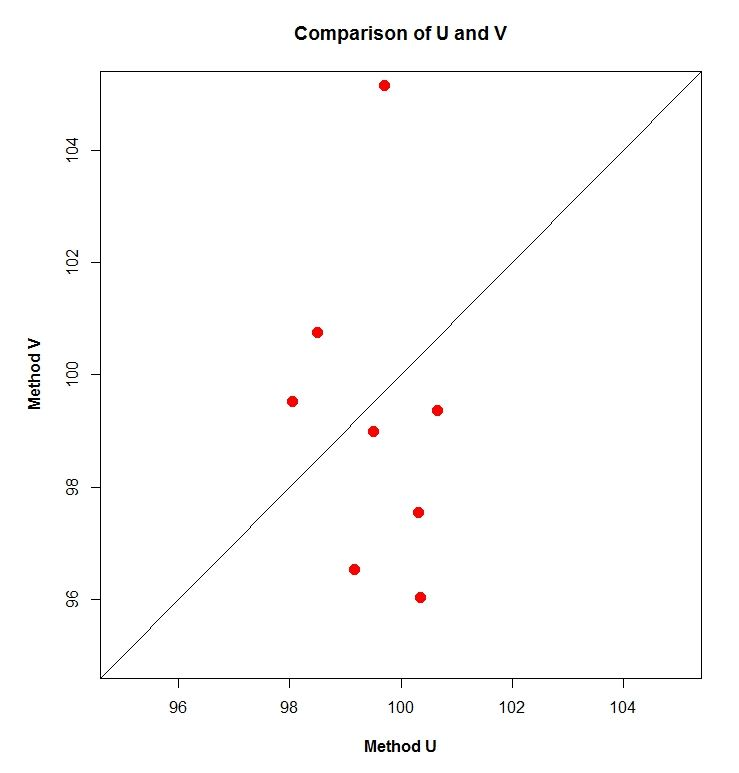
\includegraphics[width=0.7\linewidth]{EAD-UV}
		\caption{Identity Plot for example data}
		\label{fig:EADidentity}
	\end{figure}
	
	The limits of agreement are $[-9.61, 9.68]$, a wide interval for this data. As with the identity plot, this would indicate lack of agreement. As with inter-method bias, an EAD value close to zero is desirable. However, from table ~\ref{EADdata}, the EAD can be computed as 3.71. The Bland-Altman plot remains a useful part of the analysis. In \ref{fig:EAD1}, it is clear there is a systematic decrease in differences across the range of measurements.
	\begin{figure}
		\centering
		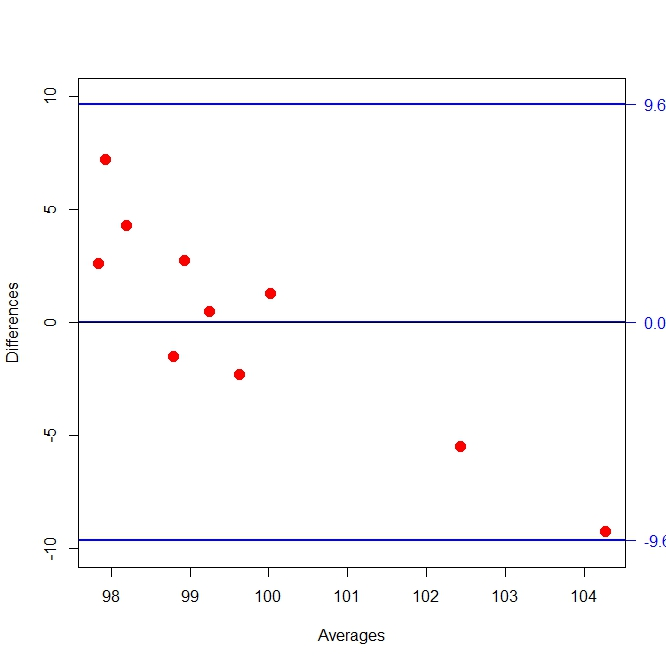
\includegraphics[width=0.7\linewidth]{images/EAD1}
		\caption{Bland-Altman Plot for UV comparison}
		\label{fig:EAD1}
	\end{figure}
	
	\citet{Barnhart} remarks that a comparison of EAD and MSD , using
	simulation studies, would be interesting, while further adding
	that `\textit{It will be of interest to investigate the benefits of these
		possible new unscaled agreement indices}'. For the Grubbs' `F vs C' and `F vs T' comparisons, the inter-method bias, difference variances, limits of agreement and EADs are shown
	in Table 1.5. The corresponding Bland-Altman plots for `F vs C' and `F vs T' comparisons were depicted previously on Figure 1.3. While the inter-method bias for the `F vs T' comparison is smaller, the EAD penalizes the comparison for having a greater variance of differences. Hence the EAD values for both comparisons are much closer.
	\begin{table}[ht]
		\begin{center}
			\begin{tabular}{|c|c|c|}
				\hline
				& F vs C & F vs T  \\
				\hline
				Inter-method bias & -0.61 & 0.12 \\ \hline
				Difference variance & 0.06 & 0.22  \\ \hline 
				Limits of agreement & (-1.08,	-0.13) & (-0.81,1.04) \\
				EAD & 0.61 & 0.35  \\ \hline 
				\hline
			\end{tabular}
			\caption{Agreement indices for Grubbs' data comparisons.}
		\end{center}
	\end{table}
	
	Further to  \citet{lin2000} and \citet{lin2002}, individual agreement between two measurement methods may be
	assessed using the the coverage probability (CP) criteria or the total deviation index (TDI). If $d_{0}$ is predetermined as the maximum acceptable absolute difference between two methods of measurement, the probability that the absolute difference of two measures being less than $d_{0}$ can be computed. This is known as the coverage probability (CP).
	
	\begin{equation}
		CP = P(|x_{i} - y_{i}| \leq d_{0})
	\end{equation}
	
	If $\pi_{0}$ is set as the predetermined coverage probability, the
	boundary under which the proportion of absolute differences is
	$\pi_{0}$ may be determined. This boundary is known as the `total
	deviation index' (TDI). Hence the TDI is the $100\pi_{0}$
	percentile of the absolute difference of paired observations.

	\section{Alternative agreement indices}
	As an alternative to limits of agreement, \citet{lin2002} proposes the use of
	the mean square deviation is assessing agreement. The mean square
	deviation is defined as the expectation of the squared differences
	of two readings . The MSD is usually used for the case of two
	measurement methods $X$ and $Y$ , each making one measurement for
	the same subject, and is given by
	\[
	MSDxy = E[(x - y)^2]  = (\mu_{x} - \mu_{y})^2 + (\sigma_{x} -
	\sigma_{y})^2 + 2\sigma_{x}\sigma_{y}(1-\rho_{xy}).
	\]
	
	
	\citet{Barnhart} advises the use of a predetermined upper limit
	for the MSD value, $MSD_{ul}$, to define satisfactory agreement.
	However, a satisfactory upper limit may not be properly
	determinable, thus creating a drawback to this methodology.
	
	
	\citet{Barnhart} proposes both the use of the square root of the
	MSD or the expected absolute difference (EAD) as an alternative agreement indices. Both of these indices can be interpreted intuitively, being denominated in the same units of measurements as the original
	measurements. Also they can be compare to the maximum acceptable
	absolute difference between two methods of measurement $d_{0}$.
	\[
	EAD = E(|x - y|) = \frac{\sum |x_{i}- y_{i}|}{n}
	\]
	
	The EAD can be used to supplement the inter-method bias in an
	initial comparison study, as the EAD is informative as a measure
	of dispersion, is easy to calculate and requires no distributional
	assumptions.
	
	\citet{Barnhart} remarks that a comparison of EAD and MSD , using
	simulation studies, would be interesting, while further adding
	that `It will be of interest to investigate the benefits of these
	possible new unscaled agreement indices'. For the Grubbs' `F vs C' and `F vs T' comparisons, the inter-method bias, difference variances, limits of agreement and EADs are shown
	in Table 1.5. The corresponding Bland-Altman plots for `F vs C' and `F vs T' comparisons were depicted previously on Figure 1.3. While the inter-method bias for the `F vs T' comparison is smaller, the EAD penalizes the comparison for having a greater variance of differences. Hence the EAD values for both comparisons are much closer.
	\begin{table}[ht]
		\begin{center}
			\begin{tabular}{|c|c|c|}
				\hline
				& F vs C & F vs T  \\
				\hline
				Inter-method bias & -0.61 & 0.12 3 \\
				Difference variances & 0.06 & 0.22  \\
				Limits of agreement & (-1.08,	-0.13) & (-0.81,1.04) \\
				EAD & 0.61 & 0.35  \\
				\hline
			\end{tabular}
			\caption{Agreement indices for Grubbs' data comparisons.}
		\end{center}
	\end{table}
	
	Further to  \citet{lin2000} and \citet{lin2002}, individual agreement between two measurement methods may be
	assessed using the the coverage probability (CP) criteria or the total deviation index (TDI). If $d_{0}$ is predetermined as the maximum acceptable absolute difference between two methods of measurement, the probability that the absolute difference of two measures being less than $d_{0}$ can be computed. This is known as the coverage probability (CP).
	
	\begin{equation}
		CP = P(|x_{i} - y_{i}| \leq d_{0})
	\end{equation}
	
	If $\pi_{0}$ is set as the predetermined coverage probability, the
	boundary under which the proportion of absolute differences is
	$\pi_{0}$ may be determined. This boundary is known as the `total
	deviation index' (TDI). Hence the TDI is the $100\pi_{0}$
	percentile of the absolute difference of paired observations.
	
	

\section{Implementation in R}
To implement an LME model in \texttt{R}, the \texttt{nlme} package is used. This package is loaded into the \texttt{R} environment using the library command, (i.e.\ \texttt{library(nlme)}). The \texttt{lme} command is used to fit LME models. The first two arguments to the \texttt{lme} function specify the fixed effect component of the model, and the data set to which the model is to be fitted. The first candidate model (`MCS1') fits an LME model on the data set `dat'. The variable `method' is assigned as the fixed effect, with the response variable `BP' (i.e.\ blood pressure).

The third argument contain the random effects component of the formulation, describing the random effects, and their grouping structure. The \texttt{nlme} package provides a set of positive-definite matrices , the \texttt{pdMat} class, that can be used to specify a structure for the between-subject variance-covariance matrix for the random effects. For Roy's methodology, we will use the \texttt{pdSymm} and \texttt{pdCompSymm} to specify a symmetric structure and a compound symmetry structure respectively. A full discussion of these structures can be found in \citet[pg. 158]{PB}.

Similarly a variety of structures for the with-subject variance-covariance matrix can be implemented using \texttt{nlme}. To implement a particular matrix structure, one must specify both a variance function and correlation structure accordingly. Variance functions are used to model the variance structure of the within-subject errors. \texttt{varIdent} is a variance function object used to allow different variances according to the levels of a classification factor in the data. A compound symmetry structure is implemented using the \texttt{corCompSymm} class, while the symmetric form is specified by \texttt{corSymm} class. Finally, the estimation methods is specified as ``ML" or ``REML".
\bigskip
The first of Roy's candidate model can be implemented using the following code;\\

\begin{framed}
	\begin{verbatim}
	MCS1 = lme(BP ~ method-1, data = dat,
	random =  list(subject=pdSymm(~ method-1)),
	weights=varIdent(form=~1|method),
	correlation = corSymm(form=~1 | subject/obs), method="ML")
	\end{verbatim}
\end{framed}

For the blood pressure data used in \citet{ARoy2009}, all four candidate models are implemented by slight variations of this piece of code, specifying either \texttt{pdSymm} or \texttt{pdCompSymm} in the second line, and either \texttt{corSymm} or \texttt{corCompSymm} in the fourth line.
For example, the second candidate model `MCS2' is implemented with the same code as MCS1, except for the term \texttt{pdCompSymm} in the second line, rather than \texttt{pdSymm}.

\begin{framed}
	\begin{verbatim}
	MCS2 = lme(BP ~ method-1, data = dat,
	random = list(subject=pdCompSymm(~ method-1)),
	weights = varIdent(form=~1|method),
	correlation = corSymm(form=~1 | subject/obs), method="ML")
	\end{verbatim}
\end{framed}

Using this \texttt{R} implementation for other data sets requires that the data set is structured appropriately (i.e.\ each case of observation records the index, response, method and replicate). Once formatted properly, implementation is simply a case of re-writing the first line of code, and computing the four candidate models accordingly.


To perform a likelihood ratio test for two candidate models, simply use the \texttt{anova} command with the names of the candidate models as arguments. The following piece of code implement the first of Roy's variability tests.

\begin{framed}
	\begin{verbatim}
	> anova(MCS1,MCS2)
	Model df    AIC    BIC  logLik   Test L.Ratio p-value
	MCS1     1  8 4077.5 4111.3 -2030.7
	MCS2     2  7 4075.6 4105.3 -2030.8 1 vs 2 0.15291  0.6958
	>
	\end{verbatim}
\end{framed}

The fixed effects estimates are the same for all four candidate models. The inter-method bias can be easily determined by inspecting a summary of any model. The summary presents estimates for all of the important parameters, but not the complete variance-covariance matrices (although some simple \texttt{R} functions can be written to overcome this). The variance estimates for the random effects for MCS2 is presented below.

\begin{framed}
	\begin{verbatim}
	Random effects:
	Formula: ~method - 1 | subject
	Structure: Compound Symmetry
	StdDev Corr
	methodJ  30.765
	methodS  30.765 0.829
	Residual  6.115
	\end{verbatim}
\end{framed}
\vspace{1cm}
Similarly, for computing the limits of agreement the standard deviation of the differences is not explicitly given. Again, A simple \texttt{R} function can be written to calculate the limits of agreement directly.

%------------------------------------------------------------------------------------%



\section{Demonstration of Roy's testing}
Roy provides three case studies, using data sets well known in method comparison studies, to demonstrate how the methodology should be used. The first two examples used are from the `blood pressure' data set introduced by \citet{BA99}. The data set is a tabulation of simultaneous measurements of systolic blood pressure were made by each of two experienced observers (denoted `J' and `R') using a sphygmomanometer and by a semi-automatic blood pressure monitor (denoted `S'). Three sets of readings were made in quick succession. Roy compares the `J' and `S' methods in his first example, and the `R' and `S' methods in his second.



%--------------------------------------------------%
\subsection{Matrix structures}
Before discussing the tests, it is useful to point out the difference between symmetric form and compound symmetry form. Consider a generic matrix $A$,

\begin{equation}
\boldsymbol{A} = \left( \begin{array}{cc}
a_{11} & a_{12}  \\
a_{21} & a_{22}  \\
\end{array}\right).
\end{equation}

A symmetric matrix allows the diagonal terms $a_{11}$ and $a_{22}$ to differ.
The compound symmetry structure requires that both of these terms be equal, i.e $a_{11} = a_{22}$.

%--------------------------------------------------%
\subsection{Variability test 1}
This is a test on whether both methods $A$ and $B$ have the same between-subject variability or not.
\begin{eqnarray}
H_{0}: \mbox{ }d_{A}  = d_{B} \\
H_{A}: \mbox{ }d_{A}  \neq d_{B}
\end{eqnarray}
When implemented using \texttt{R}, this test is facilitated by constructing a model specifying a symmetric form for $D$ (i.e. the alternative model) and comparing it with a model that has compound symmetric form for $D$ (i.e. the null model). For this test $\boldsymbol{\hat{\Lambda}}$ has a symmetric form for both models, and will be the same for both.

%--------------------------------------------------%
\subsubsection{Bland-Altman's blood data}
With the alternative model, the MLE of the between-subject variance covariance matrix is given by
\begin{equation}
\boldsymbol{\hat{D}_{Symm}} = \left( \begin{array}{cc}
923.98 & 785.24  \\
785.24 & 971.30  \\
\end{array}\right)
\end{equation}

With the null model the MLE is as follows:

\begin{equation}
\boldsymbol{\hat{D}_{CS}} = \left( \begin{array}{cc}
946.50 & 784.32  \\
784.32 & 946.50  \\
\end{array}\right)
\end{equation}
A likelihood ratio test is perform to determine which model is more suitable. The outcome of this test is presented in the following \texttt{R} code.
\begin{verbatim}
> anova(MCS1,MCS2)
>
>
Model df    AIC    BIC  logLik   Test L.Ratio p-value
MCS1     1  8 4077.5 4111.3 -2030.7
MCS2     2  7 4075.6 4105.3 -2030.8 1 vs 2 0.15291  0.6958
\end{verbatim}

The test statistic is the difference of the $-2$ log likelihoods; $0.15291$. The $p-$value is $0.6958$. Therefore we fail to reject the hypothesis that both have the same between-subject variabilities.

%---------------------------------------------%
\subsection{Variability test 2}

This is a test on whether both methods $A$ and $B$ have the same within-subject variability or not.

\begin{eqnarray}
H_{0}: \mbox{ }\lambda_{A}  = \lambda_{B} \\
H_{A}: \mbox{ }\lambda_{A}  = \lambda_{B}
\end{eqnarray}

This model is performed in the same manner as the first test, only reversing the roles of $\boldsymbol{\hat{D}}$ and $\boldsymbol{\hat{\Lambda}}$. The null model is constructed  a symmetric form for $\boldsymbol{\hat{\Lambda}}$ while the alternative model uses a compound symmetry form. This time $\boldsymbol{\hat{D}}$ has a symmetric form for both models, and will be the same for both.


\subsubsection{Bland-Altman's blood data}
For the null model the MLE of the within-subject variance covariance matrix is given below.

\begin{equation}
\boldsymbol{\hat{\Lambda}_{Symm}} = \left( \begin{array}{cc}
37.40 & 16.06  \\
16.06 & 83.14  \\
\end{array}\right)
\end{equation}
With the alternative model the MLE is as follows:

\begin{equation}
\boldsymbol{\hat{\Lambda}_{CS}} = \left( \begin{array}{cc}
60.27  & 16.06  \\
16.06  & 60.27  \\
\end{array}\right)
\end{equation}

A likelihood ratio test is perform to determine which model is more suitable.
The outcome of this test is that it can be assumed that they have equal
The test statistic is the difference of the $-2$ log likelihoods; $28.617$. The $p-$value is less than $0.0001$. In this case we reject the null hypothesis that both models have the same within-subject variabilities.

%-----------------------------------------------%
\subsection{Variability test 3}
This is a test on whether both methods $A$ and $B$ have the same overall variability or not.
\begin{eqnarray}
H_{0}: \mbox{ }\sigma_{A}  = \sigma_{B} \\
H_{A}: \mbox{ }\sigma_{A}  = \sigma_{B}
\end{eqnarray}

The null model is constructed a symmetric form for both $\boldsymbol{\hat{D}}$ and $\boldsymbol{\hat{\Lambda}}$ while the alternative model uses a compound symmetry form for both.

\subsubsection{Bland-Altman's blood data}
With the null model the MLE of the within-subject variance covariance matrix is given below.

\begin{equation}
\boldsymbol{\hat{\Sigma}_{Symm}} = \left( \begin{array}{cc}
961.38 & 801.40  \\
801.40 & 1054.43  \\
\end{array}\right)
\end{equation}

With the alternative model the MLE is as follows:
\begin{equation}
\boldsymbol{\hat{\Sigma}_{CS}} = \left( \begin{array}{cc}
1007.92  & 801.65  \\
801.65  & 1007.92  \\
\end{array}\right)
\end{equation}

Again a likelihood ratio test is used to determine the most suitable of the two candidate models.
The test statistic is the difference of the $-2$ log likelihoods; $28.884$. The $p-$value is less than $0.0001$. We again reject the null hypothesis. Each model has a different overall variability, a foregone conclusion from the second variability test.



\subsection{Test for inter-method bias}
The inter-method bias between the two method is found to be $15.62$ , with a $p-$value of

\subsection{Correlation Test}
\begin{equation}
\boldsymbol{\hat{r}_{\Omega}}_{ii} = \left( \begin{array}{cc}
1  & 0.7959  \\
0.7959  & 1  \\
\end{array}\right)
\end{equation}

The  diagonal blocks $\boldsymbol{\hat{r}_{\Omega}}_{ii}$ of the correlation matrix indicate an overall coefficient of $0.7959$.
This is less than the threshold of 0.82 that Roy recommends.

The off diagonal blocks of the overall correlation matrix $\boldsymbol{\hat{r}_{\Omega}}_{ii'}$ are
\begin{equation}
\boldsymbol{\hat{r}_{\Omega}}_{ii'} = \left( \begin{array}{cc}
0.9611  & 0.7799  \\
0.7799  & 0.9212  \\
\end{array}\right).
\end{equation}

\subsection{Conclusion of procedure}
The overall conclusion of the procedure is that the two methods are not in agreement, specifically due to the within-subject variability, and the inter-method bias. The repeatability coefficients are substantially different, one being 49\% larger than the other. Additionally the overall correlation coefficient did not exceed the recommended threshold of $0.82$.

%------------------------------------------------------------------------------------%
\newpage
\section{Demonstration of Roy's testing}
Roy provides three case studies, using data sets well known in method comparison studies, to demonstrate how the methodology should be used. The first two examples used are from the `blood pressure' data set introduced by \citet{BA99}. The data set is a tabulation of simultaneous measurements of systolic blood pressure were made by each of two experienced observers (denoted `J' and `R') using a sphygmomanometer and by a semi-automatic blood pressure monitor (denoted `S'). Three sets of readings were made in quick succession. Roy compares the `J' and `S' methods in the first of her examples.

The inter-method bias between the two method is found to be $15.62$ , with a $t-$value of $-7.64$, with a $p-$value of less than $0.0001$. Consequently there is a significant inter-method bias present between methods $J$ and $S$, and the first of the Roy's three agreement criteria is unfulfilled.

Next, the first variability test is carried out, yielding maximum likelihood estimates of the between-subject variance covariance matrix, for both the null model, in compound symmetry (CS) form, and the alternative model in symmetric (symm) form. These matrices are determined to be as follows;
\[
\boldsymbol{\hat{D}}_{CS} = \left( \begin{array}{cc}
946.50 & 784.32  \\
784.32 & 946.50  \\
\end{array}\right),
\hspace{1.5cm}
\boldsymbol{\hat{D}}_{Symm} = \left( \begin{array}{cc}
923.98 & 785.24  \\
785.24 & 971.30  \\
\end{array}\right).
\]

A likelihood ratio test is perform to compare both candidate models. The log-likelihood of the null model is $-2030.7$, and for the alternative model $-2030.8$. The test statistic, presented with greater precision than the log-likelihoods, is $0.1592$. The $p-$value is $0.6958$. Consequently we fail to reject the null model, and by extension, conclude that the hypothesis that methods $J$ and $S$ have the same between-subject variability. Thus the second of the criteria is fulfilled.

The second variability test determines maximum likelihood estimates of the within-subject variance covariance matrix, for both the null model, in CS form, and the alternative model in symmetric form.

\[
\boldsymbol{\hat{\Lambda}_{CS}} = \left( \begin{array}{cc}
60.27  & 16.06  \\
16.06  & 60.27  \\
\end{array}\right),
\hspace{1.5cm}
\boldsymbol{\hat{\Lambda}}_{Symm} = \left( \begin{array}{cc}
37.40 & 16.06  \\
16.06 & 83.14  \\
\end{array}\right).
\]

Again, A likelihood ratio test is perform to compare both candidate models. The log-likelihood of the alternative model model is $-2045.0$. As before, the null model has a log-likelihood of $-2030.7$. The test statistic is computed as $28.617$, again presented with greater precision. The $p-$value is less than $0.0001$. In this case we reject the null hypothesis of equal within-subject variability. Consequently the third of Roy's criteria is unfulfilled.
The coefficient of repeatability for methods $J$ and $S$ are found to be 16.95 mmHg and 25.28 mmHg respectively.

The last of the three variability tests is carried out to compare the overall variabilities of both methods.
With the null model the MLE of the within-subject variance covariance matrix is given below. The overall variabilities for the null and alternative models, respectively, are determined to be as follows;
\[
\boldsymbol{\hat{\Sigma}}_{CS} = \left( \begin{array}{cc}
1007.92  & 801.65  \\
801.65  & 1007.92  \\
\end{array}\right),
\hspace{1.5cm}
\boldsymbol{\hat{\Sigma}}_{Symm} = \left( \begin{array}{cc}
961.38 & 801.40  \\
801.40 & 1054.43  \\
\end{array}\right),
\]

The log-likelihood of the alternative model model is $-2045.2$, and again, the null model has a log-likelihood of $-2030.7$. The test statistic is $28.884$, and the $p-$value is less than $0.0001$. The null hypothesis, that both methods have equal overall variability, is rejected. Further to the second variability test, it is known that this difference is specifically due to the difference of within-subject variabilities.

Lastly, Roy considers the overall correlation coefficient. The diagonal blocks $\boldsymbol{\hat{r}_{\Omega}}_{ii}$ of the correlation matrix indicate an overall coefficient of $0.7959$. This is less than the threshold of 0.82 that Roy recommends.

\[
\boldsymbol{\hat{r}_{\Omega}}_{ii} = \left( \begin{array}{cc}
1  & 0.7959  \\
0.7959  & 1  \\
\end{array}\right)
\]

The off-diagonal blocks of the overall correlation matrix $\boldsymbol{\hat{r}_{\Omega}}_{ii'}$ present the correlation coefficients further to \citet{hamlett}.
\[
\boldsymbol{\hat{r}_{\Omega}}_{ii'} = \left( \begin{array}{cc}
0.9611  & 0.7799  \\
0.7799  & 0.9212  \\
\end{array}\right).
\]

The overall conclusion of the procedure is that method $J$ and $S$ are not in agreement, specifically due to the within-subject variability, and the inter-method bias. The repeatability coefficients are substantially different, with the coefficient for method $S$ being 49\% larger than for method $J$. Additionally the overall correlation coefficient did not exceed the recommended threshold of $0.82$.



\section{Worked Eamples:LikelihoodRatio Tests}

Conventionally LME models can be tested using Likelihood Ratio Tests, wherein a reference model is compared to a nested model.
\begin{framed}
	\begin{verbatim}
	> Ref.Fit = lme(y ~ meth-1, data = dat,   #Symm , Symm#
	+     random = list(item=pdSymm(~ meth-1)), 
	+     weights=varIdent(form=~1|meth),
	+     correlation = corSymm(form=~1 | item/repl), 
	+     method="ML")
	\end{verbatim}
\end{framed}
Roy(2009) presents two nested models that specify the condition of equality as required, with a third nested model for an additional test. There three formulations share the same structure, and can be specified by making slight alterations of the code for the Reference Model.
Nested Model (Between-Item Variability)
\begin{framed}
	\begin{verbatim}
	> NMB.fit  = lme(y ~ meth-1, data = dat,   #CS , Symm#
	+     random = list(item=pdCompSymm(~ meth-1)),
	+     correlation = corSymm(form=~1 | item/repl), 
	+     method="ML")
	\end{verbatim}
\end{framed}



\begin{framed}
	\begin{verbatim}
	Nested Model (Within ?item Variability)
	> NMW.fit = lme(y ~ meth-1, data = dat,   #Symm , CS# 
	+     random = list(item=pdSymm(~ meth-1)),
	+     weights=varIdent(form=~1|meth), 
	+     correlation = corCompSymm(form=~1 | item/repl), 
	+     method="ML")
	\end{verbatim}
\end{framed}

Nested Model (Overall Variability)
Additionally there is a third nested model, that can be used to test overall variability, substantively a a joint test for between-item and within-item variability. The motivation for including such a test in the suite is not clear, although it does circumvent the need for multiple comparison procedures in certain circumstances, hence providing a simplified procedure for non-statisticians.

\begin{framed}
	\begin{verbatim}
	> NMO.fit = lme(y ~ meth-1, data = dat,   #CS , CS# 
	+     random = list(item=pdCompSymm(~ meth-1)), 
	+     correlation = corCompSymm(form=~1 | item/repl), 
	+     method="ML")
	\end{verbatim}
\end{framed}

ANOVAs  for  Original Fits
The likelihood Ratio test is very simple to implement in R. All that is required it to specify the reference model and the relevant nested mode as arguments to the command anova().
The figure below displays the three tests described by Roy (2009).

\begin{framed}
	\begin{verbatim}
	> testB    = anova(Ref.Fit,NMB.fit)                          # Between-Subject Variabilities
	> testW   = anova(Ref.Fit,NMW.fit)                        # Within-Subject Variabilities
	> testO     = anova(Ref.Fit,NMO.fit)                        # Overall Variabilities
	
	\end{verbatim}
\end{framed}




%-----------------------------------------------------------------------------------------------------%
\newpage



\newpage   
\begin{verbatim}
> anova(MCS1,MCS2)
>
>
Model df    AIC    BIC  logLik   Test L.Ratio p-value
MCS1     1  8 4077.5 4111.3 -2030.7
MCS2     2  7 4075.6 4105.3 -2030.8 1 vs 2 0.15291  0.6958
\end{verbatim}

\subsection{Roy's Reference Model}
Conventionally LME models can be tested using Likelihood Ratio Tests, wherein a reference model is compared to a nested model.
\begin{framed}
	\begin{verbatim}
	> Ref.Fit = lme(y ~ meth-1, data = dat,   #Symm , Symm#
	+     random = list(item=pdSymm(~ meth-1)), 
	+     weights=varIdent(form=~1|meth),
	+     correlation = corSymm(form=~1 | item/repl), 
	+     method="ML")
	\end{verbatim}
\end{framed}


Roy(2009) presents two nested models that specify the condition of equality as required, with a third nested model for an additional test. There three formulations share the same structure, and can be specified by making slight alterations of the code for the Reference Model.

\subsection{Nested Model (Between-Item Variability)}
\begin{framed}
	\begin{verbatim}
	> NMB.fit  = lme(y ~ meth-1, data = dat,   #CS , Symm#
	+     random = list(item=pdCompSymm(~ meth-1)),
	+     correlation = corSymm(form=~1 | item/repl), 
	+     method="ML")
	\end{verbatim}
\end{framed}


\newpage
\section{Fat Data Examples: LoAs for Carstensen's data}




\citet{BXC2008} presents a data set `fat', which is a comparison of measurements of subcutaneous fat
by two observers at the Steno Diabetes Center, Copenhagen. Measurements are in millimeters
(mm). Each person is measured three times by each observer. The observations are considered to be `true' replicates.

A linear mixed effects model is formulated, and implementation through several software packages is demonstrated.
All of the necessary terms are presented in the computer output. The limits of agreement are therefore,
\begin{equation}
0.0449  \pm 1.96 \times  \sqrt{2 \times 0.0596^2 + 0.0772^2 + 0.0724^2} = (-0.220,  0.309).
\end{equation}

\citet{BXC2008} describes the calculation of the limits of agreement (with the inter-method bias implicit) for both data sets, based on his formulation;

\[\hat{\alpha}_1 - \hat{\alpha}_2 \pm 2\sqrt{2\hat{\tau}^2 +\hat{\sigma}_1^2 +\hat{\sigma}_2^2 }.\]

For the `Fat' data set, the inter-method bias is shown to be $0.045$. The limits of agreement are $(-0.23 , 0.32)$



For Carstensen's `fat' data, the limits of agreement computed using Roy's
method are consistent with the estimates given by \citet{BXC2008}; $0.044884  \pm 1.96 \times  0.1373979 = (-0.224,  0.314).$






\section{HBA1C Diabetes Example}
\citet{BXC2008} describes the sampling method when discussing of a motivating example

Diabetes patients attending an outpatient clinic in Denmark have their $HbA_{1c}$ levels routinely measured at every visit. Venous and Capillary blood samples were obtained from all patients appearing at the clinic over two days. Samples were measured on four consecutive days on each machines, hence there are five analysis days.

\citet{BXC2008} notes that every machine was calibrated every day to  the manufacturers guidelines.
Measurements are classified by method, individual and replicate. In this case the replicates are clearly not exchangeable, neither within patients nor simulataneously for all patients.


%	\citet{Roy2006} uses the ``Blood" data set, which featured in \citet{BA99}.

%=========================================================================== %
\section{Oximetry Data}
\citet{BXC2008} introduces a second data set; the oximetry study. This study done at the Royal Children�s Hospital in
Melbourne to assess the agreement between co-oximetry and pulse oximetry in small babies.

In most cases, measurements were taken by both method at three different times. In some cases there are either one or two pairs of measurements, hence the data is unbalanced. \citet{BXC2008} describes many of the children as being very sick, and with very low oxygen saturations levels. Therefore it must be assumed that a biological change can occur in interim periods, and measurements are not true replicates.

\citet{BXC2008} proposes the addition of an random effects term to their model when the replicates are linked. This term is used to describe the `item by replicate' interaction, which is independent of the methods. This interaction is a source of variability independent of the methods. Therefore failure to account for it will result in variability being wrongly attributed to the methods.

%=========================================================================== %

Limits of agreement are determined using Roy's methodology, without adding any additional terms, are found to be consistent with the `interaction' model; $(-9.562, 14.504 )$. Roy's methodology assumes that replicates are linked. However, following Carstensen's example, an addition interaction term is added to the implementation of Roy's model to assess the effect, the limits of agreement estimates do not change. However there is a conspicuous difference in within-subject matrices of Roy's model and the modified model (denoted $1$ and $2$ respectively);

Carstensen demonstrates the use of the interaction term when computing the limits of agreement for the `Oximetry' data set. When the interaction term is omitted, the limits of agreement are $(-9.97, 14.81)$. Carstensen advises the inclusion of the interaction term for linked replicates, and hence the limits of agreement are recomputed as $(-12.18,17.12)$.


Limits of agreement are determined using Roy's methodology, without adding any additional terms, are found to be consistent with the `interaction' model; $(-9.562, 14.504 )$. Roy's methodology assumes that replicates are linked. However, following Carstensen's example, an addition interaction term is added to the implementation of Roy's model to assess the effect, the limits of agreement estimates do not change. However there is a conspicuous difference in within-subject matrices of Roy's model and the modified model (denoted $1$ and $2$ respectively);
%	\begin{equation}
%	\hat{\boldsymbol{\Lambda}}_{1}= \begin{pmatrix}{
%		16.61 &	11.67\cr
%		11.67 & 27.65 }\qquad
%	\boldsymbol{\hat{\Lambda}}_{2}= \begin{pmatrix}{
%		7.55 & 2.60 \cr
%		2.60 & 18.59}.
%	\end{equation}

\noindent (The variance of the additional random effect in model $2$ is $3.01$.)

\citet{akaike} introduces the Akaike information criterion ($AIC$), a model
selection tool based on the likelihood function. Given a data set, candidate models
are ranked according to their AIC values, with the model having the lowest AIC being considered the best fit.Two candidate models can said to be equally good if there is a difference of less than $2$ in their AIC values.

The Akaike information criterion (AIC) for both models are $AIC_{1} = 2304.226$ and $AIC_{2} = 2306.226$ , indicating little difference in models. The AIC values for the Carstensen `unlinked' and `linked' models are $1994.66$ and $1955.48$ respectively, indicating an improvement by adding the interaction term.

The $\boldsymbol{\hat{\Lambda}}$ matrices are informative as to the difference between Carstensen's unlinked and linked models. For the oximetry data, the covariance terms (given above as 11.67 and 2.6 respectively ) are of similar magnitudes to the variance terms. Conversely for the `fat' data the covariance term ($-0.00032$) is negligible. When the interaction term is added to the model, the covariance term remains negligible. (For the `fat' data, the difference in AIC values is also approximately $2$).

To conclude, Carstensen's models provided a rigorous way to determine limits of agreement, but don't provide for the computation of $\boldsymbol{\hat{D}}$ and $\boldsymbol{\hat{\Lambda}}$. Therefore the test's proposed by \citet{ARoy2009} can not be implemented. Conversely, accurate limits of agreement as determined by Carstensen's model may also be found using Roy's method. Addition of the interaction term erodes the capability of Roy's methodology to compare candidate models, and therefore shall not be adopted.

Finally, to complement the blood pressure (i.e.`J vs S') method comparison from the previous section (i.e.`J vs S'), the limits of agreement are $15.62 \pm 1.96 \times 20.33 = (-24.22, 55.46)$.)


\citet{BXC2008} demonstrate the necessity of accounting for linked replicated by comparing the limits of agreement from the `oximetry' data set using a model with the additional term, and one without. When the interaction is accounted for the limits of agreement are (-9.62,14.56). When the interaction is not accounted for, the limits of agreement are (-11.88,16.83). It is shown that the failure to include this additional term results in an over-estimation of the standard deviations of differences.


\citet{BXC2008} demonstrates the use of the interaction term when computing the limits of agreement for the `Oximetry' data set. When the interaction term is omitted, the limits of agreement are $(-9.97, 14.81)$. Carstensen advises the inclusion of the interaction term for linked replicates, and hence the limits of agreement are recomputed as $(-12.18,17.12)$.

\section{Linked replicates}

\citet{BXC2008} proposes the addition of an random effects term to their model when the replicates are linked. This term is used to describe the `item by replicate' interaction, which is independent of the methods. This interaction is a source of variability independent of the methods. Therefore failure to account for it will result in variability being wrongly attributed to the methods.

\citet{BXC2008} introduces a second data set; the oximetry study. This study done at the Royal Children�s Hospital in
Melbourne to assess the agreement between co-oximetry and pulse oximetry in small babies.

In most cases, measurements were taken by both method at three different times. In some cases there are either one or two pairs of measurements, hence the data is unbalanced. \citet{BXC2008} describes many of the children as being very sick, and with very low oxygen saturations levels. Therefore it must be assumed that a biological change can occur in interim periods, and measurements are not true replicates.

\citet{BXC2008} demonstrate the necessity of accounting for linked replicated by comparing the limits of agreement from the `oximetry' data set using a model with the additional term, and one without. When the interaction is accounted for the limits of agreement are (-9.62,14.56). When the interaction is not accounted for, the limits of agreement are (-11.88,16.83). It is shown that the failure to include this additional term results in an over-estimation of the standard deviations of differences.

Limits of agreement are determined using Roy's methodology, without adding any additional terms, are found to be consistent with the `interaction' model; $(-9.562, 14.504 )$. Roy's methodology assumes that replicates are linked. However, following Carstensen's example, an addition interaction term is added to the implementation of Roy's model to assess the effect, the limits of agreement estimates do not change. However there is a conspicuous difference in within-subject matrices of Roy's model and the modified model (denoted $1$ and $2$ respectively);
\begin{equation}
	\hat{\boldsymbol{\Lambda}}_{1}= \left(\begin{array}{cc}
		16.61 &	11.67\\
		11.67 & 27.65 \end{array}\right) \qquad
	\boldsymbol{\hat{\Lambda}}_{2}= \left( \begin{array}{cc}
		7.55 & 2.60 \\
		2.60 & 18.59 \end{array} \right).
\end{equation}

\noindent (The variance of the additional random effect in model $2$ is $3.01$.)

\citet{akaike} introduces the Akaike information criterion ($AIC$), a model
selection tool based on the likelihood function. Given a data set, candidate models
are ranked according to their AIC values, with the model having the lowest AIC being considered the best fit.Two candidate models can said to be equally good if there is a difference of less than $2$ in their AIC values.

The Akaike information criterion (AIC) for both models are $AIC_{1} = 2304.226$ and $AIC_{2} = 2306.226$ , indicating little difference in models. The AIC values for the Carstensen `unlinked' and `linked' models are $1994.66$ and $1955.48$ respectively, indicating an improvement by adding the interaction term.

The $\boldsymbol{\hat{\Lambda}}$ matrices are informative as to the difference between Carstensen's unlinked and linked models. For the oximetry data, the covariance terms (given above as 11.67 and 2.6 respectively ) are of similar magnitudes to the variance terms. Conversely for the `fat' data the covariance term ($-0.00032$) is negligible. When the interaction term is added to the model, the covariance term remains negligible. (For the `fat' data, the difference in AIC values is also approximately $2$).

To conclude, Carstensen's models provided a rigorous way to determine limits of agreement, but don't provide for the computation of $\boldsymbol{\hat{D}}$ and $\boldsymbol{\hat{\Lambda}}$. Therefore the test's proposed by \citet{roy} can not be implemented. Conversely, accurate limits of agreement as determined by Carstensen's model may also be found using Roy's method. Addition of the interaction term erodes the capability of Roy's methodology to compare candidate models, and therefore shall not be adopted.

Finally, to complement the blood pressure (i.e.`J vs S') method comparison from the previous section (i.e.`J vs S'), the limits of agreement are $15.62 \pm 1.96 \times 20.33 = (-24.22, 55.46)$.)
%========================================================================================%
\newpage
\section{Alternative agreement indices}
As an alternative to limits of agreement, \citet{lin2002} proposes the use of
the mean square deviation is assessing agreement. The mean square
deviation is defined as the expectation of the squared differences
of two readings . The MSD is usually used for the case of two
measurement methods $X$ and $Y$ , each making one measurement for
the same subject, and is given by
\[
MSDxy = E[(x - y)^2]  = (\mu_{x} - \mu_{y})^2 + (\sigma_{x} -
\sigma_{y})^2 + 2\sigma_{x}\sigma_{y}(1-\rho_{xy}).
\]


\citet{Barnhart} advises the use of a predetermined upper limit
for the MSD value, $MSD_{ul}$, to define satisfactory agreement.
However, a satisfactory upper limit may not be properly
determinable, thus creating a drawback to this methodology.


\citet{Barnhart} proposes both the use of the square root of the
MSD or the expected absolute difference (EAD) as an alternative agreement indices. Both of these indices can be interpreted intuitively, being denominated in the same units of measurements as the original
measurements. Also they can be compare to the maximum acceptable
absolute difference between two methods of measurement $d_{0}$.
\[
EAD = E(|x - y|) = \frac{\sum |x_{i}- y_{i}|}{n}
\]

The EAD can be used to supplement the inter-method bias in an
initial comparison study, as the EAD is informative as a measure
of dispersion, is easy to calculate and requires no distributional
assumptions.

\citet{Barnhart} remarks that a comparison of EAD and MSD , using
simulation studies, would be interesting, while further adding
that `It will be of interest to investigate the benefits of these
possible new unscaled agreement indices'. For the Grubbs' `F vs C' and `F vs T' comparisons, the inter-method bias, difference variances, limits of agreement and EADs are shown
in Table 1.5. The corresponding Bland-Altman plots for `F vs C' and `F vs T' comparisons were depicted previously on Figure 1.3. While the inter-method bias for the `F vs T' comparison is smaller, the EAD penalizes the comparison for having a greater variance of differences. Hence the EAD values for both comparisons are much closer.
\begin{table}[ht]
	\begin{center}
		\begin{tabular}{|c|c|c|}
			\hline
			& F vs C & F vs T  \\
			\hline
			Inter-method bias & -0.61 & 0.12 3 \\
			Difference variances & 0.06 & 0.22  \\
			Limits of agreement & (-1.08,	-0.13) & (-0.81,1.04) \\
			EAD & 0.61 & 0.35  \\
			\hline
		\end{tabular}
		\caption{Agreement indices for Grubbs' data comparisons.}
	\end{center}
\end{table}

Further to  \citet{lin2000} and \citet{lin2002}, individual agreement between two measurement methods may be
assessed using the the coverage probability (CP) criteria or the total deviation index (TDI). If $d_{0}$ is predetermined as the maximum acceptable absolute difference between two methods of measurement, the probability that the absolute difference of two measures being less than $d_{0}$ can be computed. This is known as the coverage probability (CP).

\begin{equation}
CP = P(|x_{i} - y_{i}| \leq d_{0})
\end{equation}

If $\pi_{0}$ is set as the predetermined coverage probability, the
boundary under which the proportion of absolute differences is
$\pi_{0}$ may be determined. This boundary is known as the `total
deviation index' (TDI). Hence the TDI is the $100\pi_{0}$
percentile of the absolute difference of paired observations.





\section{Limits of agreement for Carstensen's data}


\citet{bxc2008} describes the calculation of the limits of agreement (with the inter-method bias implicit) for both data sets, based on his formulation;

\[\hat{\alpha}_1 - \hat{\alpha}_2 \pm 2\sqrt{2\hat{\tau}^2 +\hat{\sigma}_1^2 +\hat{\sigma}_2^2 }.\]

For the `Fat' data set, the inter-method bias is shown to be $0.045$. The limits of agreement are $(-0.23 , 0.32)$

Carstensen demonstrates the use of the interaction term when computing the limits of agreement for the `Oximetry' data set. When the interaction term is omitted, the limits of agreement are $(-9.97, 14.81)$. Carstensen advises the inclusion of the interaction term for linked replicates, and hence the limits of agreement are recomputed as $(-12.18,17.12)$.




\subsection{RV-IV}
For the the RV-IC comparison, $\hat{D}$ is given by


\begin{equation}
	\hat{D}= \left[ \begin{array}{cc}
		1.6323 & 1.1427  \\
		1.1427 & 1.4498 \\
	\end{array} \right]
\end{equation}

The estimate for the within-subject variance covariance matrix is
given by
\begin{equation}
	\hat{\Sigma}= \left[ \begin{array}{cc}
		0.1072 & 0.0372  \\
		0.0372 & 0.1379  \\
	\end{array}\right]
\end{equation}
The estimated overall variance covariance matrix for the the 'RV
vs IC' comparison is given by
\begin{equation}
	Block \Omega_{i}= \left[ \begin{array}{cc}
		1.7396 & 1.1799  \\
		1.1799 & 1.5877  \\
	\end{array} \right].
\end{equation}

The power of the likelihood ratio test may depends on specific sample size and the
specific number of  replications, and the author proposes simulation studies to examine this further.
%===============================================================================================================%
\section{LME - Pankaj Choudhury}
Consistent with the conventions of mixed models, \citep{pkc}
formulates the measurement $y_{ij} $from method $i$ on individual
$j$ as follows;
\begin{equation}
y_{ij} =P_{ij}\theta + W_{ij}v_{i} + X_{ij}b_{j} + Z_{ij}u_{j} +
\epsilon_{ij},     (j=1,2, i=1,2....n)
\end{equation}
The design matrix $P_{ij}$ , with its associated column vector
$\theta$, specifies the fixed effects common to both methods. The
fixed effect specific to the $j$th method is articulated by the
design matrix $W_{ij}$ and its column vector $v_{i}$. The random
effects common to both methods is specified in the design matrix
$X_{ij}$, with vector $b_{j}$ whereas the random effects specific
to the $i$th subject by the $j$th method is expressed by $Z_{ij}$,
and vector $u_{j}$. Noticeably this notation is not consistent
with that described previously.  The design matrices are specified
so as to includes a fixed intercept for each method, and a random
intercept for each individual. Additional assumptions must also be
specified;
\begin{equation}
v_{ij} \sim N(0,\Sigma),
\end{equation}
These vectors are assumed to be independent for different $i$s,
and are also mutually independent. All Covariance matrices are
positive definite.  In the above model effects can be classed as
those common to both methods, and those that vary with method.
When considering differences, the effects common to both
effectively cancel each other out. The differences of each pair of
measurements can be specified as following;
\begin{equation}
d_{ij} = X_{ij}b_{j} + Z_{ij}u_{j} + \epsilon_{ij},     (j=1,2,
i=1,2....n)
\end{equation}
This formulation has seperate distributional assumption from the
model stated previously.

This agreement covariate $x$ is the key step in how this
methodology assesses agreement.
%%%%%%%%%%%%%%%%%%%%%%%%%%%%%%%%%%%%%%%%%%%%%%%%%%%%%%%%%%%%%%%%%%%%%%%%%%%%%%%%%%%%%%%%%%%%%%%%%%%%%%%5
%----------------------------------------------------------------------------%
\newpage

	\newpage
	\section{The Hat Matrix} %5.1
	
	The projection matrix $H$ (also known as the hat matrix), is a
	well known identity that maps the fitted values $\hat{Y}$ to the
	observed values $Y$, i.e. $\hat{Y} = HY$.
	
	\begin{equation}
	H =\quad X(X^{T}X)^{-1}X^{T}
	\end{equation}
	
	$H$ describes the influence each observed value has on each fitted
	value. The diagonal elements of the $H$ are the `leverages', which
	describe the influence each observed value has on the fitted value
	for that same observation. The residuals ($R$) are related to the
	observed values by the following formula:
	\begin{equation}
	R = (I-H)Y
	\end{equation}
	
	The variances of $Y$ and $R$ can be expressed as:
	\begin{eqnarray}
	\mbox{var}(Y) = H\sigma^{2} \nonumber\\
	\mbox{var}(R) = (I-H)\sigma^{2}
	\end{eqnarray}
	
	Updating techniques allow an economic approach to recalculating
	the projection matrix, $H$, by removing the necessity to refit the
	model each time it is updated. However this approach is known for
	numerical instability in the case of down-dating.
	
	
	\section{Cross Validation} %5.4
	
	Cross validation techniques for linear regression employ the use `leave one out' re-calculations. In such procedures the regression coefficients are estimated for $n-1$ covariates, with the $Q^{th}$ observation omitted.
	
	Let $\hat{\beta}$ denote the least square estimate of $\beta$ based upon the full set of observations, and let
	$\hat{\beta}^{-Q}$ denoted the estimate with the $Q^{th}$ case
	excluded.
	
	
	In leave-one-out cross validation, each observation is omitted in turn, and a regression model is fitted on the rest of the data. Cross validation is used to estimate the generalization error of a given model. alternatively it can be used for model selection by determining the candidate model that has the smallest generalization error.
	
	
	Evidently leave-one-out cross validation has similarities with `jackknifing', a well known statistical technique. However cross validation is used to estimate generalization error, whereas the jackknife technique is used to estimate bias.
	
	\subsection{Cross Validation: Updating standard deviation} %5.4.1
	
	The variance of a data set can be calculated using the following formula.
	\begin{equation}
	S^{2}=\frac{\sum_{i=1}^{n}(x_{i}^{2})-\frac{(\sum_{i=1}^{n}x_{i})^{2}}{n}}{n-1}
	\end{equation}
	
	While using bivariate data, the notation $Sxx$ and $Syy$ shall apply to the variance of $x$ and of $y$ respectively. The covariance term $Sxy$ is given by
	
	\begin{equation}
	Sxy=\frac{\sum_{i=1}^{n}(x_{i}y_{i})-\frac{(\sum_{i=1}^{n}x_{i})(\sum_{i=1}^{n}y_{i})}{n}}{n-1}
	\end{equation}
	
	Let the observation $j$ be omitted from the data set. The estimates for the variance identities can be updating using minor adjustments to the full sample estimates. Where $(j)$ denotes that the $j$th has been omitted, these identities are
	
	\begin{equation}
	Sxx^{(j)}=\frac{\sum_{i=1}^{n}(x_{i}^{2})-(x_{j})^{2}-\frac{((\sum_{i=1}^{n}x_{i})-x_{j})^{2}}{n-1}}{n-2}
	\end{equation}
	\begin{equation}
	Syy^{(j)}=\frac{\sum_{i=1}^{n}(y_{i}^{2})-(y_{j})^{2}-\frac{((\sum_{i=1}^{n}y_{i})-y_{j})^{2}}{n-1}}{n-2}
	\end{equation}
	\begin{equation}
	Sxy^{(j)}=\frac{\sum_{i=1}^{n}(x_{i}y_{i})-(y_{j}x_{j})-\frac{((\sum_{i=1}^{n}x_{i})-x_{j})(\sum_{i=1}^{n}y_{i})-y_{k})}{n-1}}{n-2}
	\end{equation}
	
	The updated estimate for the slope is therefore
	\begin{equation}
	\hat{\beta}_{1}^{(j)}=\frac{Sxy^{(j)}}{Sxx^{(j)}}
	\end{equation}
	
	It is necessary to determine the mean for $x$ and $y$ of the
	remaining $n-1$ terms
	\begin{equation}
	\bar{x}^{(j)}=\frac{(\sum_{i=1}^{n}x_{i})-(x_{j})}{n-1},
	\end{equation}
	
	\begin{equation}
	\bar{y}^{(j)}=\frac{(\sum_{i=1}^{n}y_{i})-(y_{j})}{n-1}.
	\end{equation}
	
	The updated intercept estimate is therefore
	
	\begin{equation}
	\hat{\beta}_{0}^{(j)}=\bar{y}^{(j)}-\hat{\beta}_{1}^{(j)}\bar{x}^{(j)}.
	\end{equation}
	
	%------------------------------------------------------------------------%
	\newpage
	\section{Updating Estimates} %5.5
	
	\subsection{Updating of Regression Estimates}
	Updating techniques are used in regression analysis to add or delete rows from a model, allowing the analyst the effect of the observation associated with that row. In time series problems, there will be scientific interest in the changing relationship between variables. In cases where there a single row is to be added or deleted, the procedure used is equivalent to a geometric rotation of a plane.
	
	Updating techniques are used in regression analysis to add or delete rows from a model, allowing the analyst the effect of the observation associated with that row.
	
	\subsection{Updating Standard deviation}
	A simple, but useful, example of updating is the updating of the standard deviation when an observation is omitted, as practised in statistical process control analyzes. From first principles, the variance of a data set can be calculated using the following formula.
	\begin{equation}
	S^{2}=\frac{\sum_{i=1}^{n}(x_{i}^{2})-\frac{(\sum_{i=1}^{n}x_{i})^{2}}{n}}{n-1}
	\end{equation}
	
	While using bivariate data, the notation $Sxx$ and $Syy$ shall apply hither to the variance of $x$ and of $y$ respectively. The covariance term $Sxy$ is given by
	
	\begin{equation}
	Sxy=\frac{\sum_{i=1}^{n}(x_{i}y_{i})-\frac{(\sum_{i=1}^{n}x_{i})(\sum_{i=1}^{n}y_{i})}{n}}{n-1}.
	\end{equation}
	
	\subsection{Updating of Regression Estimates}
	Updating techniques are used in regression analysis to add or
	delete rows from a model, allowing the analyst the effect of the
	observation associated with that row. In time series problems,
	there will be scientific interest in the changing relationship
	between variables. In cases where there a single row is to be
	added or deleted, the procedure used is equivalent to a geometric
	rotation of a plane.
	
	Consider a $p \times p$ matrix $X$, from which a row $x_{i}^{T}$
	is to be added or deleted. \citet{CookWeisberg} sets $A = X^{T}X$,
	$a=-x_{i}^{T}$ and $b=x_{i}^{T}$, and writes the above equation as
	
	\begin{equation}
	(X^{T}X \pm x_{i}x_{i}^{T})^{-1} = \quad(X^{T}X )^{-1} \mp \quad
	\frac{(X^{T}X)^{-1}(x_{i}x_{i}^{T}(X^{T}X)^{-1}}{1-x_{i}^{T}(X^{T}X)^{-1}x_{i}}
	\end{equation}
	
	\subsection{Updating Regression Estimates}
	Let the observation $j$ be omitted from the data set. The estimates for the variance identities can be updating using minor adjustments to the full sample estimates. Where $(j)$ denotes that the $j$th has been omitted, these identities are
	
	\begin{equation}
	Sxx^{(j)}=\frac{\sum_{i=1}^{n}(x_{i}^{2})-(x_{j})^{2}-\frac{((\sum_{i=1}^{n}x_{i})-x_{j})^{2}}{n-1}}{n-2}
	\end{equation}
	\begin{equation}
	Syy^{(j)}=\frac{\sum_{i=1}^{n}(y_{i}^{2})-(y_{j})^{2}-\frac{((\sum_{i=1}^{n}y_{i})-y_{j})^{2}}{n-1}}{n-2}
	\end{equation}
	\begin{equation}
	Sxy^{(j)}=\frac{\sum_{i=1}^{n}(x_{i}y_{i})-(y_{j}x_{j})-\frac{((\sum_{i=1}^{n}x_{i})-x_{j})(\sum_{i=1}^{n}y_{i})-y_{k})}{n-1}}{n-2}
	\end{equation}
	
	The updated estimate for the slope is therefore
	\begin{equation}
	\hat{\beta}_{1}^{(j)}=\frac{Sxy^{(j)}}{Sxx^{(j)}}
	\end{equation}
	
	It is necessary to determine the mean for $x$ and $y$ of the
	remaining $n-1$ terms
	\begin{equation}
	\bar{x}^{(j)}=\frac{(\sum_{i=1}^{n}x_{i})-(x_{j})}{n-1},
	\end{equation}
	
	\begin{equation}
	\bar{y}^{(j)}=\frac{(\sum_{i=1}^{n}y_{i})-(y_{j})}{n-1}.
	\end{equation}
	
	The updated intercept estimate is therefore
	
	\begin{equation}
	\hat{\beta}_{0}^{(j)}=\bar{y}^{(j)}-\hat{\beta}_{1}^{(j)}\bar{x}^{(j)}.
	\end{equation}
	
	\subsection{Inference on intercept and slope}
	\begin{equation}
	\hat{\beta_{1}} \pm t_{(\alpha, n-2) }
	\sqrt{\frac{S^2}{(n-1)S^{2}_{x}}}
	\end{equation}
	
	\begin{equation}
	\frac{\hat{\beta_{0}}-\beta_{0}}{SE(\hat{\beta_{0}})}
	\end{equation}
	\begin{equation}
	\frac{\hat{\beta_{1}}-\beta_{1}}{SE(\hat{\beta_{0}})}
	\end{equation}
	
	
	\subsubsection{Inference on correlation coefficient} This test of
	the slope is coincidentally the equivalent of a test of the
	correlation of the $n$ observations of $X$ and $Y$.
	\begin{eqnarray}
	H_{0}: \rho_{XY} = 0 \nonumber \\
	H_{A}: \rho_{XY} \ne 0 \nonumber \\
	\end{eqnarray}
	
%------------------------------------------------------------------------%
\section{residuals.lme {nlme}- Extract lme Residuals}

The residuals at level $i$ are obtained by subtracting the fitted levels at that level from the response vector (and dividing by the estimated within-group standard error, if \texttt{type="pearson"}). 

The fitted values at level i are obtained by adding together the population fitted values (based only on the fixed effects estimates) and the estimated contributions of the random effects to the fitted values at grouping levels less or equal to i.

%------------------------------------------------------------------------%

\begin{framed}
	\begin{verbatim}
	
	fm1 <- lme(distance ~ age + Sex, 
	data = Orthodont, random = ~ 1)
	head(residuals(fm1, level = 0:1))
	summary(residuals(fm1) /
	residuals(fm1, type = "p")) 
	
	# constant scaling factor 1.432
	
	\end{verbatim}
\end{framed}


\section{influence.ME}

\textit{influence.ME} allows you to compute measures of influential data for mixed effects models generated by lme4.

\textit{influence.ME} provides a collection of tools for detecting influential cases in generalized mixed effects models. It analyses models that were estimated using lme4. The basic rationale behind identifying influential data is that when iteratively single units are omitted from the data, models based on these data should not produce substantially different estimates. 

To standardize the assessment of how influential a (single group of) observation(s) is, several measures of influence are common practice, such as DFBETAS and Cook's Distance. In addition, we provide a measure of percentage change of the fixed point estimates and a simple procedure to detect changing levels of significance.
\subsection{Influence() command}
\texttt{influence()} is the workhorse function of the influence.ME package. Based on a priorly estimated mixed effects regression model (estimated using lme4), the \texttt{influence()} function iteratively modifies the mixed effects model to neutralize the effect a grouped set of data has on the parameters, and which returns returns the fixed parameters of these iteratively modified models. These are used to compute measures of influential data.


\subsection{Classical Model}
The classical model is based on measurements $y_{mi}$
by method $m=1,2$ on item $i = 1,2 \ldots$

\[y_{mi} + \alpha_{m} + \mu_{i} + e_{mi}\]

\[e_{mi} \sim \mathcal{n} (0,\sigma^2_m)\]

Even though the separate variances can not be
identified, their sum can be estimated by the empirical variance of the differences.

Like wise the separate $\alpha$ can not be
estimated, only theiir difference can be estimated as
$\bar{D}$

\section{Lai Shiao}

\citet{LaiShiao} advocates the use of LME models to study method comparison problems. The authors analyse a data set typical of method comparison studies using SAS software, with particular use of the \emph{`Proc Mixed'} package. The stated goal of this study is to determine which factor from a specified group of factors is the key contributor to the difference in the two methods.

The study relates to oxygen saturation, the most investigated variable in clinical nursing studies \citep{LaiShiao}. The two method compared are functional saturation (SO2, percent functional oxy-hemoglobin) and fractional saturation (HbO2, percent fractional oxy-hemoglobin), which is considered to be the `gold standard' method of measurement.

\citet{LaiShiao} establishes an LME model for analysing the differences $D_{ijtl}$, where $D_{ijtl}$ is the differences of the measurements (i.e = $SO2_{ijtl}$ - $HbO2_{ijtl}$) for the ith donor at the $j$th level of foetal haemoglobin percent (Fhbperct) and the $t$th repeated measurement by the $l$th practitioner of the experiment.


(\citet{BXC2004} also advocates the use of LME models in comparing methods, but with a different emphasis.)
\citet{LaiShiao} use mixed models to determine the factors that
affect the difference of two methods of measurement using the
conventional formulation of linear mixed effects models.

If the parameter \textbf{b}, and the variance components are not
significantly different from zero, the conclusion that there is no
inter-method bias can be drawn. If the fixed effects component
contains only the intercept, and a simple correlation coefficient
is used, then the estimate of the intercept in the model is the
inter-method bias. Conversely the estimates for the fixed effects
factors can advise the respective influences each factor has on
the differences. It is possible to pre-specify different
correlation structures of the variance components \textbf{G} and
\textbf{R}.


Oxygen saturation is one of the most frequently measured variables
in clinical nursing studies. `Fractional saturation' ($HbO_{2}$)
is considered to be the gold standard method of measurement, with
`functional saturation' ($SO_{2}$) being an alternative method.
The method of examining the causes of differences between these
two methods is applied to a clinical study conducted by
\citet{Shiao}. This experiment was conducted by 8 lab
practitioners on blood samples, with varying levels of
haemoglobin, from two donors. The samples have been in storage for
varying periods ( described by the variable `Bloodage') and are
categorized according to haemoglobin percentages(i.e
$0\%$,$20\%$,$40\%$,$60\%$,$80\%$,$100\%$). There are 625
observations in all.

\citet{LaiShiao} fits two models on this data, with the lab
technicians and the replicate measurements as the random effects
in both models. The first model uses haemoglobin level as a fixed
effects component. For the second model, blood age is added as a
second fixed factor.

\subsubsection{Single fixed effect} The first model fitted by \citet{LaiShiao} takes the
blood level as the sole fixed effect to be analyzed. The following
coefficient estimates are estimated by `Proc Mixed';
\begin{eqnarray}
	\mbox{fixed effects :   } 2.5056 - 0.0263\mbox{Fhbperct}_{ijtl} \\
	(\mbox{p-values :   } = 0.0054, <0.0001, <0.0001)\nonumber\\\nonumber\\
	\mbox{random effects :   } u(\sigma^{2}=3.1826) + e_{ijtl}
	(\sigma^{2}_{e}=0.1525, \rho= 0.6978) \nonumber\\
	(\mbox{p-values :   } = 0.8113, <0.0001, <0.0001)\nonumber
\end{eqnarray}

With the intercept estimate being both non-zero and statistically
significant ($p=0.0054$), this models supports the presence
inter-method bias is $2.5\%$ in favour of $SO_{2}$. Also, the
negative value of the haemoglobin level coefficient indicate that
differences will decrease by $0.0263\%$ for every percentage
increase in the haemoglobin .

In the random effects estimates, the variance due to the
practitioners is $3.1826$, indicating that there is a significant
variation due to technicians ($p=0.0311$) affecting the
differences. The variance for the estimates is given as $0.1525$,
($p<0.0001$).

\subsubsection{Two fixed effects}
Blood age is added as a second fixed factor to the model,
whereupon new estimates are calculated;
\begin{eqnarray}
	\mbox{fixed effects :   } -0.2866 + 0.1072 \mbox{Bloodage}_{ijtl}
	- 0.0264\mbox{Fhbperct}_{ijtl}\nonumber\\
	( \mbox{p-values :   } = 0.8113, <0.0001, <0.0001)\nonumber\\\nonumber\\
	\mbox{random effects :   } u(\sigma^{2}=10.2346) + e_{ijtl}
	(\sigma^{2}_{e}=0.0920, \rho= 0.5577) \nonumber\\
	(\mbox{p-values :   } = 0.0446, <0.0001, <0.0001)
\end{eqnarray}


With this extra fixed effect added to the model, the intercept
term is no longer statistically significant. Therefore, with the
presence of the second fixed factor, the model is no longer
supporting the presence of inter-method bias. Furthermore, the
second coefficient indicates that the blood age of the observation
has a significant bearing on the size of the difference between
both methods ($p <0.0001$). Longer storage times for blood will
lead to higher levels of particular blood factors such as MetHb
and HbCO (due to the breakdown and oxidisation of the
haemoglobin). Increased levels of MetHb and HbCO are concluded to
be the cause of the differences. The coefficient for the
haemoglobin level doesn't differ greatly from the single fixed
factor model, and has a much smaller effect on the differences.
The random effects estimates also indicate significant variation
for the various technicians; $10.2346$ with $p=0.0446$.

\citet{LaiShiao} demonstrates how that linear mixed effects models
can be used to provide greater insight into the cause of the
differences. Naturally the addition of further factors to the
model provides for more insight into the behavior of the data.

\newpage
	\section{Sherman Morrison Woodbury Formula} % 5.2
	
	The `Sherman Morrison Woodbury' Formula is a well known result in
	linear algebra;
	\begin{equation}
		(A+a^{T}B)^{-1} \quad = \quad A^{-1}-
		A^{-1}a^{T}(I-bA^{-1}a^{T})^{-1}bA^{-1}
	\end{equation}
	
	This result is highly useful for analyzing regression diagnostics,
	and for matrices inverses in general. Consider a $p \times p$
	matrix $X$, from which a row $x_{i}^{T}$ is to be added or
	deleted. \citet{CookWeisberg} sets $A = X^{T}X$, $a=-x_{i}^{T}$
	and $b=x_{i}^{T}$, and writes the above equation as
	
	\begin{equation}
		(X^{T}X \pm x_{i}x_{i}^{T})^{-1} = \quad(X^{T}X )^{-1} \mp \quad
		\frac{(X^{T}X)^{-1}(x_{i}x_{i}^{T}(X^{T}X)^{-1}}{1-x_{i}^{T}(X^{T}X)^{-1}x_{i}}
	\end{equation}
	
	The projection matrix $H$ (also known as the hat matrix), is a
	well known identity that maps the fitted values $\hat{Y}$ to the
	observed values $Y$, i.e. $\hat{Y} = HY$.
	
	\begin{equation}
		H =\quad X(X^{T}X)^{-1}X^{T}
	\end{equation}
	
	$H$ describes the influence each observed value has on each fitted value. The diagonal elements of the $H$ are the `leverages', which describe the influence each observed value has on the fitted value for that same observation. The residuals ($R$) are related to the observed values by the following formula:
	\begin{equation}
		R = (I-H)Y
	\end{equation}
	
	The variances of $Y$ and $R$ can be expressed as:
	\begin{eqnarray}
		\mbox{var}(Y) = H\sigma^{2} \nonumber\\
		\mbox{var}(R) = (I-H)\sigma^{2}
	\end{eqnarray}
	
	Updating techniques allow an economic approach to recalculating the projection matrix, $H$, by removing the necessity to refit the model each time it is updated. However this approach is known for
	numerical instability in the case of down-dating.
	
	
	
	\subsection{Hat Values for MCS regression}
	
	With A as the averages and D as the casewise differences.
	\begin{verbatim}
	fit = lm(D~A)
	\end{verbatim}
	
	\begin{displaymath}
		H = A \left(A^\top  A\right)^{-1} A^\top ,
	\end{displaymath}
	
	%------------------------------------------------------------------------%



\newpage
\bibliographystyle{chicago}
\bibliography{DB-txfrbib}
\end{document}


